\subsection{Description}
The dynamic range compressor is an effect which limits the change in audio levels, allowing for a more constant volume. This effect is used to enhance the listener's ability to hear soft vocals in an audio track or to limit large peaks in volume.

\subsection{Applications}
The Dynamic Range Compressor is oftentimes used to reduce listener's fatigue by reducing the severity of volume level transitions. Another application is to aid in speech recognition, allowing the listener to hear soft voices in the background.

\subsection{Principles of Operation}
The effect allows the user to adjust the relationship between the input and output waveforms and volume levels. As the input audio is fed in, the compressor shrinks the dynamic range of the input from 20dB in to 10dB on the output. By doing this, the transients are limited in their range.

\subsection{Implementation Notes}
To implement this effect, we used Adobe Audition due to the complex nature of a dynamic range compressor. We experimented with the curve to change this relationship. A screenshot of our compressor curves is shown in Figure \ref{fig:drc-audition}.
\begin{figure}[ht]
    \centering
    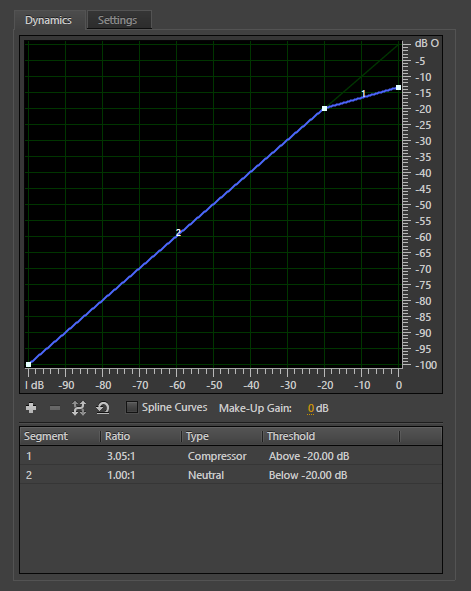
\includegraphics[scale=0.6]{drc.PNG}
    \caption{Dynamic Range Compression Settings in Adobe Audition}
    \label{fig:drc-audition}
\end{figure}

\subsection{Demo and Discussion}
We tried dynamic range compression in Adobe Audition to reduce the range from -20 dB to 0 dB into -20 dB to -10 dB (input: \href{run:../InputAudio/22-001 Original Vocal.wav}{original vocals}). You can hear the larger transients reduced in the \href{run:../OutputAudio/drc_normal.wav}{output}. However, a common failure of dynamic range compression is that it makes the output sound \href{run:../OutputAudio/drc_extreme.wav}{if overdone} (threshold set to -45 dB).

\subsection{Further Exploration}
While Dynamic Range Compression may at first sound simple, it has many moving parts which happen inside the code. After a little digging on Youtube, we were able to find \href{https://www.youtube.com/watch?v=dd4ujGjlX1k}{this video} which goes through and explains what dynamic range compressors do.